\documentclass{article}
\usepackage[utf8]{inputenc}

\title{ECE210 Final Review - Cramming Carnival Solutions}
\author{Author: Members of HKN}
\date{Fall 2024}

\newcommand{\dd}[1]{\mathrm{d}#1}
\usepackage{physics}

\renewcommand*\contentsname{Table of Contents}

\usepackage[makeroom]{cancel}
\usepackage[letterpaper, portrait, margin=1in]{geometry}
\usepackage{graphicx}

\usepackage{tikz}
\usepackage[siunitx, RPvoltages]{circuitikz}
\usepackage{xfrac}
\usepackage{circledsteps}

\usepackage{amsmath,amsthm,hyperref, amsfonts}

\usepackage{float}
\usepackage{indentfirst}

\pagenumbering{arabic}

\begin{document}

\maketitle

\pagenumbering{arabic}

\section{Fabled Fourier}

Determine the Fourier transform of the following:
\begin{enumerate}
    \item $f(t) = \text{sinc}(4t-8) * -\text{rect}(t)$
    \item $g(t) = \frac{1}{(4 + jt)^2}$
    \item $h(t) = \text{sinc}^2(3t-3)$
    \item $h'(t)$
\end{enumerate}

\subsection{Solution for 1.1:}

This looks like a difficult convolution. Let's go to the frequency domain instead. The following transforms are on the table:

$$\text{sinc}(4t) \Longleftrightarrow \frac{\pi}{4} \text{rect}\bigg(\frac{\omega}{8}\bigg)$$

$$-\text{rect}(t) \Longleftrightarrow -\text{sinc}\bigg(\frac{\omega}{2}\bigg)$$

However, the sinc function has a time shift by 2, as $\text{sinc}(4t-8) = \text{sinc}(4(t-2))$. This means we multiply the first transform by $e^{-j\omega2}$.

$$\text{sinc}(4t-8) \Longleftrightarrow \frac{\pi}{4} \text{rect}\bigg(\frac{\omega}{8}\bigg)e^{-j\omega2}$$

Convolution in time is equal to multiplication in frequency. So we simply have to multiply these two signals together.

$$F(\omega) = \bigg(\frac{\pi}{4} \text{rect}\bigg(\frac{\omega}{8}\bigg)e^{-j\omega2}\bigg)\bigg(-sinc\bigg(\frac{\omega}{2}\bigg)\bigg)$$

$$\longrightarrow \boxed{F(\omega) = -\frac{\pi}{4} \text{rect}\bigg(\frac{\omega}{8}\bigg)e^{-j\omega2}\text{sinc}\bigg(\frac{\omega}{2}\bigg)}$$

\subsection{Solution for 1.2:}

Looking through our tables, we notice that this looks a lot like the frequency side of one of the transforms. This implies that we need to use the symmetry property. Let's make a table.

\begin{center}
\begin{tabular}{||c | c | c ||} 
 \hline
 Time Domain & Frequency Domain & Step Taken  \\ [1ex] 
 \hline\hline
 $te^{-4t}u(t)$ & $\frac{1}{(4 + j\omega)^2}$ & Row 5 of the Fourier Transform Tables \\ [1ex] 
 \hline
 $\frac{1}{(4 + jt)^2}$ & $2\pi (-\omega) e^{4 \omega} u(-\omega)$ & Symmetry Property \\ [1ex] 
 \hline
\end{tabular}
\end{center}

Final answer: $\boxed{G(\omega) = -2\pi\omega e^{4 \omega} u(-\omega)}$

\subsection{Solution for 1.3:}

This one happens to be directly on the tables. We first have to change the argument from $3t-3$ to $3(t-1)$ in order to pull out the proper time shift.

The time shift adds a $e^{-j\omega}$ factor. We use $W = 6$ in row 10 of the Fourier Transform tables. Thus, we get

$$\boxed{H(\omega) = \frac{\pi}{3} \Delta \left(\frac{\omega}{12}\right) e^{-jw}}$$

Alternatively, we could've pulled apart the two sincs and transformed them into rectangles individually. Multiplication in time is convolution in frequency, so the two rectangles would then be convolved. Since we're convolving a rectangle with itself, we will end up with a triangle.

\subsection{Solution for 1.4:}

A derivative in the time domain simply becomes a multiplication by $j \omega$ in the frequency domain.

$$\boxed{H_2(\omega) = j \omega \frac{\pi}{3} \Delta \left(\frac{\omega}{12}\right) e^{-jw}}$$

\newpage

\section{Scintillating Simplifications}

Simplify the following expressions:

a. $f(t) = (t^2 + 1)\delta(t - 1)\delta(t + 1)$

b. $g(t) = (t^2 + 1)(\delta(t - 1) + \delta(t + 1))$

c. $h(t) = (t^2 + 1) * (\delta(t - 1) + \delta(t + 1))$

\subsection{Solutions:}

Part a: $$f(t) = (t^2 + 1)\delta(t - 1)\delta(t + 1)$$

The answer for this one is $\boxed{f(t) = 0}$. The two deltas being multiplied together mean that for all $t$ one of the terms in the multiplication is 0.

Part b: $$g(t) = (t^2 + 1)(\delta(t - 1) + \delta(t + 1))$$

Let's distribute first.

$$g(t) = (t^2 + 1)\delta(t - 1) + (t^2 + 1)\delta(t + 1)$$

Remember that multiplication by delta means keeping the delta and evaluating the terms in front of it at the point where the delta is nonzero (try and recall intuitively why this is!) Thus,

$$\boxed{g(t) = 2\delta(t - 1) + 2 \delta(t + 1)}$$

Part c: $$h(t) = (t^2 + 1) * (\delta(t - 1) + \delta(t + 1))$$

Convolution by delta means throwing out the delta and shifting the function by the same amount as the delta was shifted. Thus,

$$h(t) = (t-1)^2 + 1 + (t+1)^2 + 1$$

$$h(t) = t^2 - 2t + 1 + 1 + t^2 + 2t + 1 + 1$$

$$\boxed{h(t) = 2t^2 + 4}$$
\newpage

\section{Clever Components} The component represented as a box in the following problem has the following time-domain I-V relationship.

\[
V(t) = K\dv[2]{I(t)}{t}
\]

Let $v(t) = \sin(t)$, and let $K_1 = 4$. Assume all initial conditions are 0 in the circuit, aside from the driving force $v(t)$. Given the circuit below, answer the following questions.

\begin{figure}[ht!]
\centering
\begin{circuitikz}[american, transform shape, voltage dir = old]
\draw (-1,0) to[R, l_=$K_1$, european] ++ (0,-3) to[short] ++ (-3,0)
		to[V=$v(t)$] ++ (0,3) to[R, l^=$2\,\unit{\ohm}$] ++ (3,0);

\draw (-0.7,0) to[open, v=$ $] ++ (0,-3);
\node at (-0.7,-1.5) [anchor=west]{$v_x(t)$};
\end{circuitikz}
\end{figure}

\paragraph{a)} What are the units of $K$? Use at most two other units in your answer.

\subsection{Solution:} Dimensional analysis first gives us the following:

\[
\text{Volt} = \text{?} \times \frac{\text{Ampere}}{\text{second}^2}
\]

\[
\frac{\text{Volt}\cdot\text{second}^2}{\text{Ampere}} = \text{?} 
\]

Note that the unit of Volt-second-per-Ampere already has another term - namely, a Henry - since that is the unit of inductance. Therefore, in two units, we get that $K$ is in units of Henry-seconds, or $\boxed{\text{H}\cdot\text{s}}$. The equivalent answers $\boxed{\Omega\cdot\text{s}^2}$ and $\boxed{\text{s}^3\cdot\text{F}^{-1}}$ are also acceptable. 

\paragraph{b)} Find the current $i(t)$ and voltage $v_x(t)$, in the time domain, using only real functions. 

\subsection{Solution:}

We are asked to find the voltage in the time domain. The term 'steady state' is not specified, so there may be some transient behavior that also needs to be accounted for. Therefore, we should use s-domain analysis.

We can write down the time-domain KCL loop as follows:

\[
\sin(t) = 2i(t) + 2\dv[2]{i}{t}
\]

Utilizing the Laplace Transform gives us:

\[
\frac{1}{s^2+1} = 2\hat{I}(s) + 2s^2\hat{I}(s)
\]
Note that we are able to remove the $i(0)$ and $i'(0)$ terms, since we are told that all initial conditions are 0. If this was not the case, we would need to include the respective terms.
\[
\frac{1}{s^2+1} = (2+2s^2)\hat{I}(s)
\]
\[
\frac{1}{2(s^2+1)^2} = \hat{I}(s)
\]

Partial Fraction Decomposition might not work here; so we have to get a bit clever with how we approach this. For now, let's ignore the 1/2 - we can multiply it back later. Right now, the closest thing on the transform table seems to be the following:

\[
t\cos(at) = \frac{s^2 - a^2}{(s^2 + a^2)^2}
\]
Let's see if we can do something with that.

\[
at\cos(at) = \frac{as^2 - a^3}{(s^2 + a^2)^2}
\]
\[
\sin(at) = \frac{a}{s^2+a^2} = \frac{as^2 + a^3}{(s^2 + a^2)^2}
\]
\[
\sin(at) - at\cos(at) = \frac{2a^3}{(s^2 + a^2)^2}
\]

With $a = 1$, we can now pretty much directly write down what our $i(t)$ should end up being (note that we are now re-including the 1/2 that we got rid of earlier):

\[
\boxed{i(t) = \frac{1}{4}\big(\sin(t) - t\cos(t)\big)}
\]

\paragraph{Note:} This solution blows up as time goes to infinity. This makes sense if you think about the value of the coefficient $K$ - since it is greater than 1, that means that changes in $v(t)$ are being amplified with no constraint. A 'clean' second derivative component is almost entirely unrealizable in practice, and this is just a theoretical problem.

\newpage

\section{Illuminating Impulse Response}

Consider an LTI system where the input $f(t) = 5u(t)$ results in a zero-state response $y(t) = e^{5t}u(t)$. Find the impulse response of the system. Also state if the system is causal or BIBO-stable. If it isn't BIBO-stable, name a bounded input that will cause an unbounded output.

\subsection{Solution:}

For this one we can just use the derivative property (recall that derivatives pass right through a system unscathed).

$$5u(t) \longrightarrow \boxed{system} \longrightarrow e^{5t}u(t)$$

Take the derivative on both sides.

$$5\delta(t) \longrightarrow \boxed{system} \longrightarrow e^{5t}\delta(t) + 5e^{5t}u(t)$$

$$\delta(t) \longrightarrow \boxed{system} \longrightarrow \frac{1}{5}e^{5t}\delta(t) + e^{5t}u(t)$$

We can simplify the right side due to impulse properties (see question 2b). Note that the right side is our impulse response because we inputted an impulse into our sytem and that's what we got.

$$\boxed{\frac{1}{5}\delta(t) + e^{5t}u(t)}$$

The system \boxed{\text{is not BIBO-stable}} - the bounded input $5u(t)$ given in the problem produces an unbounded output $e^{5t}u(t)$. However, the system is \boxed{\text{causal}} - the impulse response is equal to 0 for all time before 0.

\vspace{3cm}

\section{Tremendous Transformations}

Q: Determine the Thevenin equivalent of the following network between nodes a and b, and then determine the available power of the network:
\vspace{-3mm}

\begin{figure}[h]
\begin{center}
    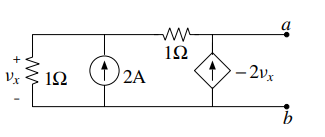
\includegraphics[width=0.4 
    \textwidth]{figures/qqqq.PNG}
\end{center}
\end{figure}

\vspace{-3mm}

\subsection{Solution:}
\newpage

The first step to solving this problem is to find $V_T$ - the open-circuit voltage. We do this in two steps - first, by applying KCL at nodes \Circled{A} and \Circled{B}, which shows us that the current through the top resistor is $-2v_x$ and the current through our left-most resistor is $2-2v_x$. Ohm's law on the top resistor gives us $v_{R1} = -2v_x$, and on the left-most resistor gives us the equation $v_x = (2-2v_x) \cdot 1$, which we solve to find that $v_x = 2/3$. 


\vspace{-3mm}

%step 1
\begin{figure}[ht!]
\centering
\ctikzset{bipoles/length=1.2cm}
\begin{circuitikz}[american,scale=0.8]

\draw (-3,3) to[R, l_=1<\ohm>, v^ = $v_x$ ] (-3,0) -- (0,0)  to[isource, l=2<\ampere>] (0,3) to[short, *-] (1,3) to[R=1<\ohm>] (3,3) to[short, -*] (5,3) ;

\draw (4,0) to[cI, l=-2$v_x$, -*] (4,3);
\draw (5,0) to[short, *-] (0,0);
\draw (0,3) to[short, i_ = $2-2v_x$] (-3,3);
\draw (5.2,3) to[open, v = $V_T$] (5.2,0);


\draw (3,2.5) to[open, v = $v_{R_1}$] (1,2.5);

\draw (1,3) to[short, i_ = $-2v_x$] (0.5,3);

\draw (0,3) node[anchor=south]{\Circled{B}};
\draw (4,3) node[anchor=south]{\Circled{A}};

\draw (5,3) node[anchor = west]{$a$};
\draw (5,0) node[anchor = west]{$b$};

\end{circuitikz}
\end{figure}

Now, we can apply KVL to loop \Circled{1} in the figure below, which gives us the following equation: $v_{R1} + v_x -V_T= 0$. Plugging in our $v_x$ and $v_{R1}$ from earlier and solving gives us $V_T = -2/3$ V.

\vspace{-3mm}

%step 2
\begin{figure}[ht!]
\centering
\ctikzset{bipoles/length=1.2cm}
\begin{circuitikz}[american, scale=0.8]

\draw (-3,3) to[R, l_=1<\ohm>, v^ = $v_x$ ] (-3,0) -- (0,0)  to[isource, l=2<\ampere>] (0,3) to[short] (1,3) to[R=1<\ohm>] (3,3) to[short, -*] (5,3) ;

\draw (4,0) to[cI, l=-2$v_x$] (4,3);
\draw (5,0) to[short, *-] (0,0);
\draw (0,3) to[short] (-3,3);
\draw (5.2,3) to[open, v = $V_T$] (5.2,0);

\draw (5,3) node[anchor = west]{$a$};
\draw (5,0) node[anchor = west]{$b$};

\draw (3,2.5) to[open, v = $v_{R_1}$] (1,2.5);

%\draw[dashed, ->] (1.5,1.5) ellipse (3.5cm and 1cm);

\draw[dashed, -latex] ($(1.5, 1.5) + (20:3.5cm and 0.75cm)$(P) arc (20:340:3.5cm and 0.75cm);
\draw (4.5, 0.5) node[anchor=mid]{\Circled{1}};
\end{circuitikz}
\end{figure}


\vspace{-3mm}

Next, we can find the Thevenin resistance using the test-signal method. We suppress our independent sources, and apply a 1 A test current to the output. KCL at node \Circled{A'} gives us that the current flowing through both resistors is $1-2v_x$. Then, Ohm's Law at the left-most resistor gives us $1-2v_x = v_x$, or that $v_x = 1/3$. \underline{Note that this is different from the $v_x$ we found earlier!} The values of dependent sources are not constant when we change the input at our two terminals. Another Ohm's Law equation also tells us that $v_{R1} = 1-2v_x$.
\vspace{-5mm}

%step 2
\begin{figure}[ht!]
\centering
\ctikzset{bipoles/length=1.2cm}
\begin{circuitikz}[american, scale=0.8]

\draw (-2,3) to[R, l_=1<\ohm>, v^ = $v_x$ ] (-2,0) -- (0,0)  to[open, o-o] (0,3) to[short,] (1,3) to[R=1<\ohm>] (3,3) to[short, -*] (6.25,3) ;

\draw (4,0) to[cI, l=-2$v_x$, -*] (4,3);
\draw (6.25,0) to[short, *-o] (0,0);
\draw (0,3) to[short,o-] (-2,3);
\draw (6.25,0) to[isource, l_= 1<\ampere>, v^=$v_{ab}$] (6.25,3);

\draw (0,3) to[short, i_=$1-2v_x$, o-] (-2,3);

\draw (6.25,3) node[anchor = west]{$a$};
\draw (6.25,0) node[anchor = west]{$b$};

\draw (4,3) node[anchor=south]{\Circled{A'}};

\draw (3,2.5) to[open, v = $v_{R_1}$] (1,2.5);

\draw[dashed, -latex] ($(2.1, 1.45) + (20:3cm and 0.8cm)$(P) arc (20:340:3cm and 0.8cm);
\draw (5, 0.5) node[anchor=mid]{\Circled{2}};

\end{circuitikz}
\end{figure}

\vspace{-3mm}

We now use a KVL equation on loop 2, getting $v_{R1} + v_x -v_{ab}= 0$ - plugging in our values from above gives us $v_{ab} = 2/3$, and then a final Ohm's Law, this time on our test-signal source, gives us that $R_{T} = v_{ab}/i_{test} = 2/3 \; \Omega$. The available power, then, is given by $\boxed{P_{avs} = \frac{V_T^2}{4R_T} = \frac{1}{6}\text{ W}}$.

\begin{figure}[ht!]
\centering
\ctikzset{bipoles/length=1.2cm}
\begin{circuitikz}[american, scale=0.75]

\draw (3,3) to[R, o-] (0,3);
 \draw (0,0) to[vsource] (0,3) ;
\draw (0,0) to[short, -o] (3,0);

\draw (3.2,3) to[open, v = $V_T$] (3.2,0);

\draw (-1.1,1.5) node[anchor=mid,]{-$\sfrac{2}{3}$ V};
\draw (1.5,3.5) node[anchor=mid]{$\sfrac{2}{3}$ $\Omega$};

\end{circuitikz}
\end{figure}

\newpage

\section{Legendary Laplace}

\begin{itemize}
    \item Find the Laplace Transform of $x(t) = e^t u(-t)$.
    \item Find the Laplace Transform of $x(t) = rect(t - \frac{1}{2})$.
\end{itemize}

\subsection{Solution:}

The first one is actually 0 for all time after 0. This means that the Laplace Transform of $x(t)$ is in fact 0. The Laplace Transform that you learn in this class is the one-sided Laplace Transform, which only handles causal signals and does not deal with signals that are nonzero before $t = 0$.

Verification: Simply use the integral. $\hat{H}_s = e^{st} \int_{0^-}^{\infty} e^{s \tau} x(\tau) d\tau = e^{st} \int_{0^-}^{\infty} e^{s \tau} 0 d\tau = 0$

\vspace{1cm}

For the second one we could do some fancy manipulations with the table. Or we can practice evaluating the actual integral.

$$\hat{X}_s = \int_{0^-}^{\infty}x(t)e^{-st}dt$$

$$\longrightarrow \int_{0}^{1}(1)e^{-st}dt$$

$$\longrightarrow \left. \frac{e^{-st}}{-s} \right\rvert^1_0$$

Note that the integral implies that $s \neq 0$.

$$\longrightarrow \frac{e^{-s} - e^{-0}}{-s}$$

$$\longrightarrow \boxed{\frac{1 - e^{-s}}{s}}$$

$s = 0$ is not allowed, but be careful! $s = 0$ isn't a pole either. Taking L'Hopital's rule will show you that this converges to 1 as $s$ goes to 0.

There is a pole at $s = -\infty$ however. Besides those values, this formula is valid for all possible $s$, so the ROC contains all of $s$.

\newpage

\section{Iconic Inverses}

\begin{itemize}
    \item Find the inverse Laplace Transform of $\hat{H}(s) = \frac{1}{s(s^2 + 2s + 2)}$.
    \item Find the inverse Laplace Transform of $\hat{H}(s) = e^{-4s}\frac{6s-1}{(s+1)^2(s-2)}$.
\end{itemize}

\subsection{Solutions:}

Recall that finding inverses is as simple as pulling apart the fraction into separate fractions.

$$\hat{H}(s) = \frac{1}{s(s^2 + 2s + 2)}$$

Factor the quadratic using the quadratic formula.

$$\longrightarrow \frac{1}{s(s-(-1 + j))(s-(-1 - j))}$$

Oh man, we have complex roots. However, the polynomial had real-valued coefficients, which means that the poles and the numerators are complex conjugate pairs as well.

$$\hat{H}(s) = \frac{A_0}{s} + \frac{A_1}{s+1-j} + \frac{A_2}{s+1+j}$$

Use the thumb-coverup rule (review this if you don't remember how! This is a very important skill!)

For the first term, we delete the first fraction and evaluate $s$ at 0.

$$A_0 = \frac{1}{(0-(-1+j))(0-(-1-j))}$$

For the second term, we delete the middle fraction and evaluate $s$ at $(-1+j)$.

$$A_1 = \frac{1}{(-1+j)(-1+j+1+j)}$$

Since the denominators are complex conjugates, we know that $A_1$ and $A_2$ are complex conjugates as well. Thus, we simplify and get

$$\hat{H}(s) = \frac{\frac{1}{2}}{s} + \frac{\frac{1}{2(-1-j)}}{s-(-1+j)} + \frac{\frac{1}{2(-1+j)}}{s-(-1-j)}$$

Now we can convert everything back to the time domain (converting each term into an exponential)

$$h(t) = \frac{1}{2} u(t) + \frac{1}{2(-1-j)}e^{(-1+j)t}u(t) + \frac{1}{2(-1+j)}e^{(-1-j)t}u(t)$$

We could be done here. However, due to the fact that we have complex exponentials that are conjugates of each other, there is some simplifying that can be done.

First, note that

$$\frac{1}{2(-1-j)} = \frac{1}{2\sqrt{2}}e^{j \frac{3\pi}{4}} \text{ and } \frac{1}{2(-1+j)} = \frac{1}{2\sqrt{2}}e^{-j \frac{3\pi}{4}}$$

Therefore, $h(t)$ now becomes

$$h(t) = \frac{1}{2}u(t) + \frac{1}{2\sqrt{2}} e^{-t}u(t) (e^{j \frac{3\pi}{4}}e^{jt} + e^{j \frac{-3\pi}{4}}e^{-jt})$$

$$\longrightarrow h(t) = \frac{1}{2}u(t) + \frac{1}{2\sqrt{2}} e^{-t}u(t) (e^{j(t +  \frac{3\pi}{4})} + e^{-j(t + \frac{3\pi}{4})})$$

$$\longrightarrow h(t) = \frac{1}{2}u(t) + \frac{1}{2\sqrt{2}} e^{-t}u(t) 2 cos(t + \frac{3 \pi}{4})$$

$$\longrightarrow h(t) = \boxed{\frac{1}{2}u(t) + \frac{1}{\sqrt{2}} e^{-t}u(t) cos(t + \frac{3 \pi}{4})}$$

\vspace{1cm}

For the second part, remember that an exponential in the $s$ domain causes a time-shift in the time domain. So we throw out the exponential and deal with it later.

We have a duplicate pole, so we need to add all powers of poles up to the power in the transform in our expansion.

$$\Hat{H}(s) = \frac{A_0}{s-2} + \frac{A_1}{s+1} + \frac{A_2}{(s+1)^2}$$

We can solve for $A_0$ and $A_2$ normally. We will solve for $A_1$ by just filling the gaps by evaluating the resulting function at some point $s$ and solving for $A_1$.

$$A_2 = \frac{6s-1}{s-2} \vert_{s = -1} = \frac{7}{3}$$

$$A_0 = \frac{6s-1}{(s+1)^2} \vert_{s = 2} = \frac{11}{9}$$

Therefore,

$$\Hat{H}(s) = \frac{6s-1}{(s+1)^2(s-2)} = \frac{\frac{11}{9}}{s-2} + \frac{A_1}{s+1} + \frac{\frac{7}{3}}{(s+1)^2}$$

Let's choose some point $s$ that isn't a pole. For convenience, let's use $s = 0$.

$$\frac{-1}{(1)^2(-2)} = \frac{\frac{11}{9}}{-2} + \frac{A_1}{1} + \frac{\frac{7}{3}}{(1)^2}$$

Solving for $A_1$, we get $A_1 = -\frac{11}{9}$.

Thus, $$\Hat{H}(s) = \frac{6s-1}{(s+1)^2(s-2)} = \frac{\frac{11}{9}}{s-2} + \frac{\frac{-11}{9}}{s+1} + \frac{\frac{7}{3}}{(s+1)^2}$$

which therefore implies that

$$h(t) = \frac{11}{9}e^{2t}u(t) - \frac{11}{9}e^{-t}u(t) + \frac{7}{3}te^{-t}u(t)$$

However, don't forget about the exponential that we tossed aside at the beginning! That exponential corresponds to a time shift by 4. Therefore the final solution is

$$\boxed{h(t) = \frac{11}{9}e^{2(t-4)}u((t-4) - \frac{11}{9}e^{-(t-4)}u((t-4)) + \frac{7}{3}(t-4)e^{-(t-4)}u((t-4))}$$

\newpage

\section{Perplexing Poles}

Determine the poles and ROC of the following transfer function, and determine if it represents a BIBO-stable LTIC system.

$$\hat{H}(s) = \frac{s^4(s + 3)}{(s^2 + 5s + 6)}$$

\subsection{Solution:}

Let's do some factoring.

$$\Hat{H}(s) = \frac{s^4(s+3)}{(s+3)(s+2)}$$

We must cancel out matching terms to find the poles and ROC.

$$\Hat{H}(s) = \frac{s^4}{(s+2)}$$

Therefore, there's a pole at $s = -2$. However, don't forget to check for poles at $\pm \infty$! In this case there are also poles at $s = \infty$ and at $s = -\infty$.

Therefore, the poles are at $\boxed{s = -2, s = \infty, s = -\infty}$.

The ROC is simply the right side of the rightmost pole, excluding the pole at $\infty$. Therefore,

$\boxed{ROC: s = \sigma + j \omega \vert \sigma > -2}$

However, BIBO-stability requires there to be no poles on the right hand plane, including the $\sigma = 0$ line. Unfortunately we have a pole at $s = \infty$. Therefore this system is $\boxed{\text{not BIBO-stable}}$.

\vspace{4cm}

\section{Evanescent Electronics}

Let $f(t)$ be the input to the following circuit, with $y(t)$ denoted as:

\begin{figure}[h]
\begin{center}
    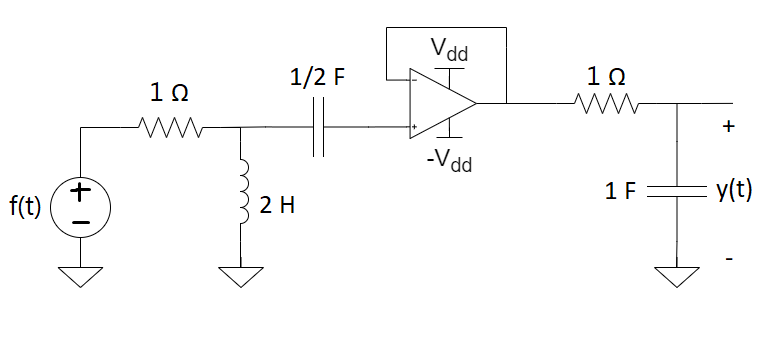
\includegraphics[width=0.5 
    \textwidth]{figures/circuit7.png}
\end{center}
\end{figure}

Find the circuit's transfer function in the time domain.

\subsection{Solution:}

We first consider the portion to the left of the operational amplifier. We convert this to the s-domain, and then convert it to a Thevenin equivalent.

\begin{figure}[h]
\begin{center}
    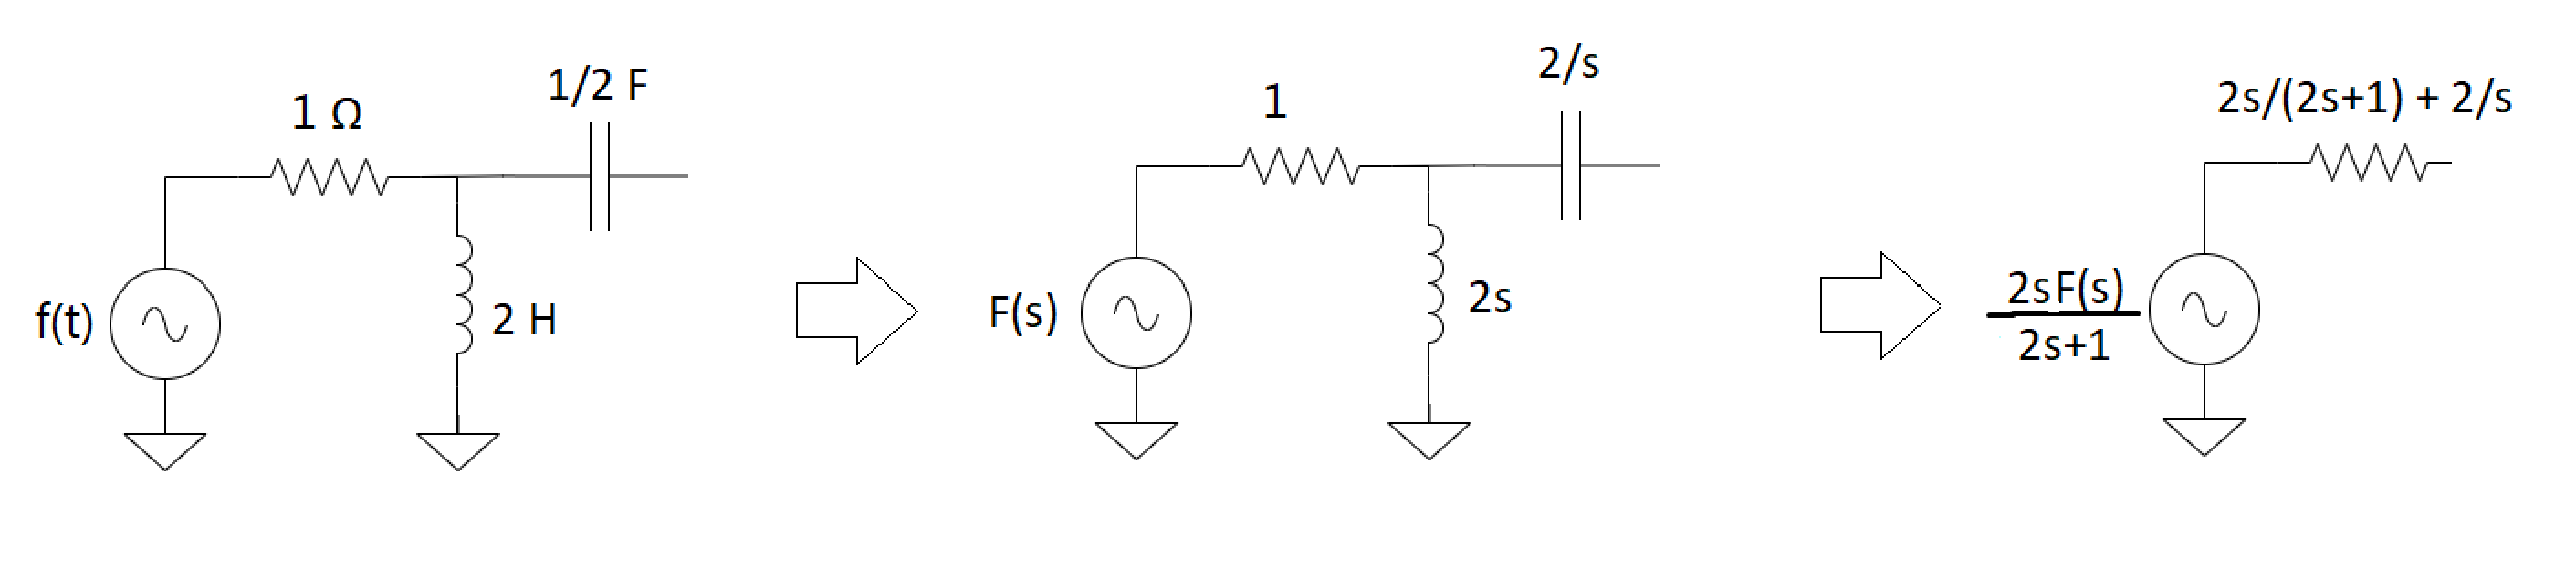
\includegraphics[width=
    \textwidth]{figures/step1.png}
\end{center}
\end{figure}

Note that you should always, always convert things into Thevenin equivalents whenever you don't know what to do! Thevenin equivalents are extremely easy to work with, and thus are an extremely powerful tool.

The next portion of this circuit is the op-amp. If you recognized this as a voltage buffer, that's great - if not, we can use the op-amp approximations to derive that fact. 

Notice that there is no input current into either input of the op-amp, and so the $v_+$ terminal has the same voltage as our Thevenin equivalent, since KCL enforces a voltage drop of 0 across the Thevenin resistance. 

Next, we can use $v_+ = v_-$ to find that the voltage on $v_-$ is the same as our Thevenin input. Since $v_+$ and $v_o$ are connected by a wire with no resistivity, their potentials are the same. As such, we see that $v_o = v_+ = \frac{2sF(s)}{2s+1}$.

Thus, our new circuit is:

\begin{figure}[h]
\begin{center}
    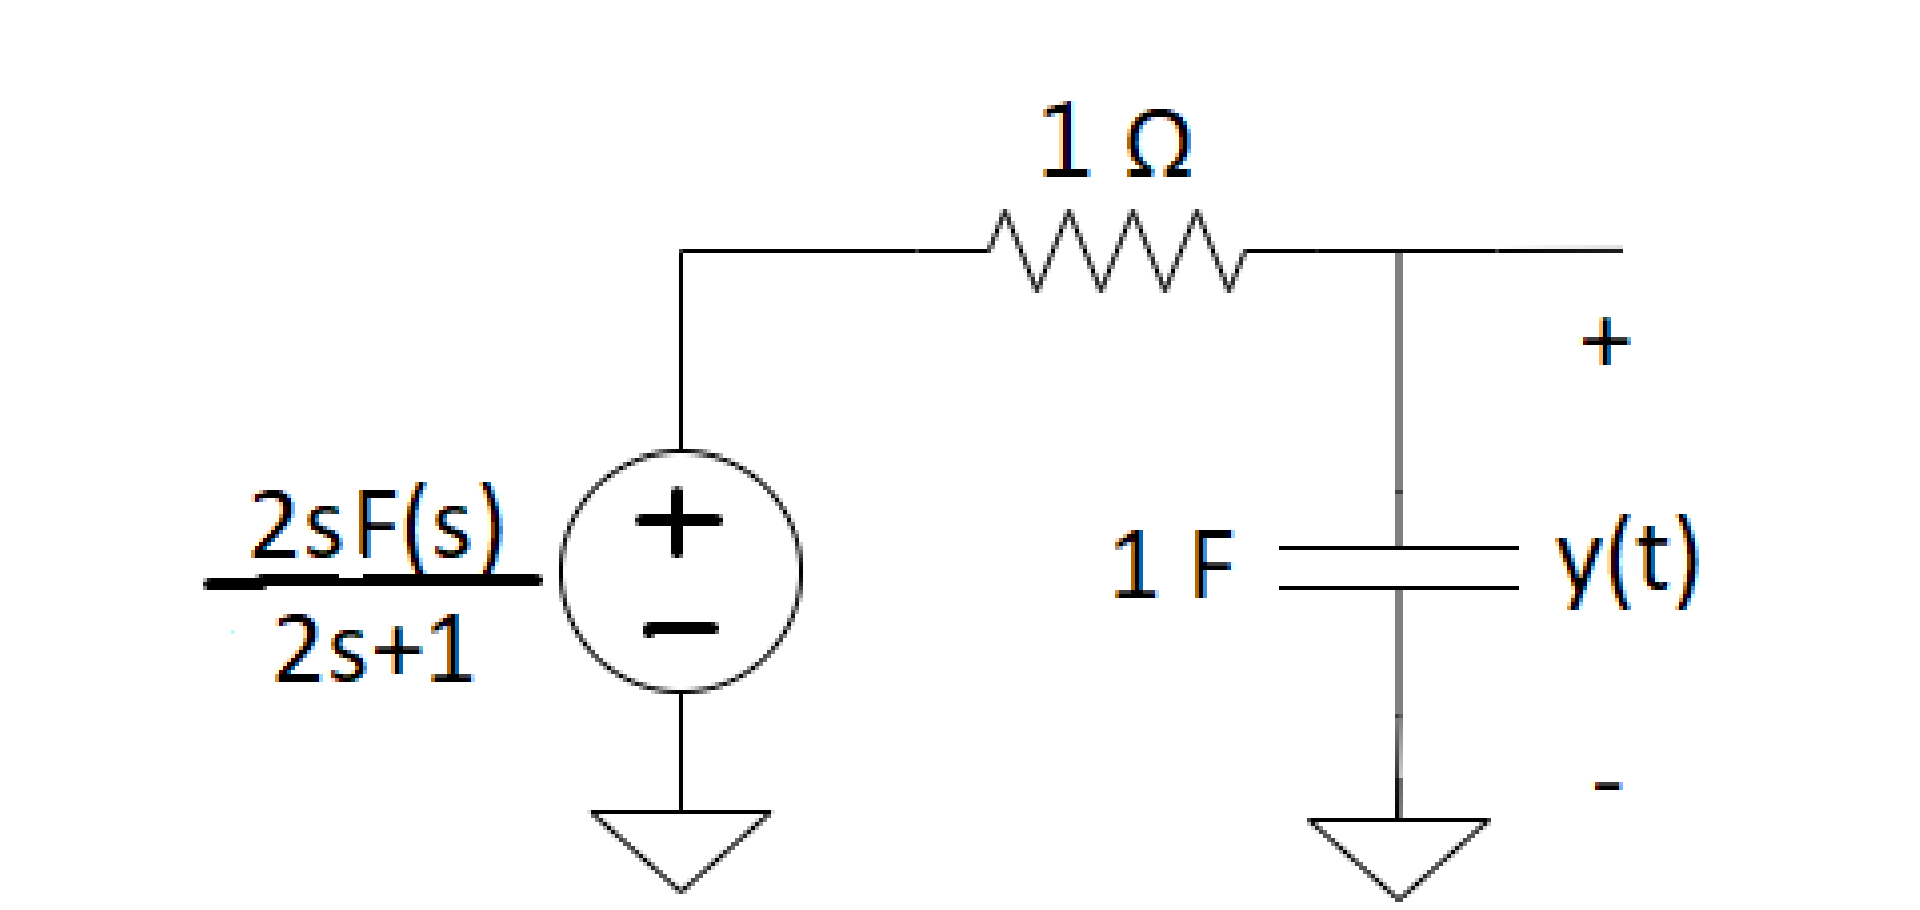
\includegraphics[width= 0.5
    \textwidth]{figures/step2.png}
\end{center}
\end{figure}

From here, we can convert again to the s-domain, where voltage division tells us that our transfer function in the s-domain is:

\[
\hat{H}(s) = \frac{Y(S)}{F(S)} = \frac{2s}{2s+1}\frac{\frac{1}{s}}{\frac{1}{s}+1} = \frac{2s}{2s+1}\frac{1}{s+1} = \frac{2s}{(2s+1)(s+1)} = \frac{2}{s+1} - \frac{2}{2s+1}
\]

We now use the Laplace Transform Tables to convert back to our time domain. This gives us:

\[
\boxed{h(t) = 2e^{-t}u(t)-e^{-t/2}u(t)}
\]

\newpage

\section{Delightful Differential}

Consider an LTIC system described by the ODE

$$\frac{d^2y}{dt^2}+\frac{dy}{dt}-2y(t) = f(t)$$

with initial conditions $y(0^-) = 3$ and $y'(0^-) = 8$.

Determine the system's transfer function $\hat{H}(s)$, its characteristic polynomial, characteristic poles, characteristic modes, and zero-input solutions in both the $s$ domain and the time domain. Also note if the system is BIBO stable or not and say why.

\subsection{Solution:}

Let's first find $\hat{H}(s)$. To do that we can discard the initial conditions completely (for now).

$$s^2Y + sY - 2Y = F$$

$$\longrightarrow \boxed{\hat{H}(s) = \frac{Y}{F} = \frac{1}{s^2 + s - 2} = \frac{1}{(s+2)(s-1)}}$$

The characteristic polynomial, poles, and modes are easy enough. We use our denominator that we found.

$$\boxed{\text{Characteristic polynomial: } s^2 + s - 2}$$

$$\boxed{\text{Characteristic poles: } s = -2, s = 1}$$

$$\boxed{\text{Characteristic modes: } e^{-2t}, e^t}$$

We have the poles, so we might as well talk about BIBO-stability now. There is a pole on the right-hand plane, so this system $\boxed{\text{is not BIBO-stable}}$.

For the zero-input solution we now need to actually consider initial conditions. Let's rewrite our ODE to include the initial conditions.

$$s^2Y - sy(0^-) - y'(0^-) + sY - y(0^-) - 2Y = F$$

$$s^2Y - 3s - 8 + sY - 3 - 2Y = F$$

$$Y(s^2 + s - 2) = F + 3s + 11$$

$$\boxed{\hat{Y}_{ZI}(s) = \frac{3s + 11}{s^2 + s - 2}}$$

\newpage

\section{Insidious Inputs}

Q: Let a system be defined by its input-output relation $y(t) = x(102841) + x(t)$. Is the system Linear? Time-Invariant? BIBO-Stable? Causal? If it is BIBO-Unstable, name a bounded input that will cause an unbounded output.

\subsection{Solution:}

\boxed{\text{Nonlinear}}. This is an example of an affine transformation, which takes the form $y = Mx + b$, where $b$ is some constant, and $M$ is some linear map. Affine transformations are 'shifts' of linear transformations but are not themselves linear. To prove this, you can test the non-linearity of this system by putting in $f(t)$ and $g(t)$ into the system separately, and then putting in $f(t)+g(t)$ as a single input. The affine shift doubles when the two inputs are put in separately, when comapred to the output.

\boxed{\text{Time-variant}}. Let's do this one formally. First we time-shift the input and then put it through our system. We'll get $x(102841 - t_0) + x(t - t_0)$. Now we put the input through our system and then time-shift. We'll get $y(t-t_0) = x(102841) + x(t-t_0)$. These two are not the same!

\boxed{\text{BIBO-Stable}}. If the input is bounded then both terms in the $y(t)$ equation are bounded, so the output itself will be bounded as well.

\boxed{\text{Noncausal}}. $y(0)$ depends on $x(0)$ and $x(102841)$, which from $t = 0$'s point of view is in the future. Note that finding some $h(t)$ and checking if $h(t) = 0$ for all negative values of $t$ is not even possible since the system isn't LTI.


\section{Outrageous Outputs}

Q: Let a system be defined by the following input-output relation:
$$y(t) =
    \begin{cases}
      9^t x(t-4) & ,-\infty \leq t \leq 10^6\\
      sin^3(t+4) cos(t+2) x(t-1) & ,10^6 < t < \infty
    \end{cases}$$    
Is the system Linear? Time-Invariant? BIBO-Stable? Causal? If it is BIBO-Unstable provide a bounded input that causes an unbounded input.

\subsection{Solution:}

\boxed{\text{Linear}}. Since time doesn't move around (that's testing for time-invariance), all $x(t)$s are multiplied by just a constant (when evaluating at each time $t$). Piecewise this system is linear, so the whole thing is linear.

\boxed{\text{Time-variant}}. If we shifted the input, the $t_0$ will only appear in the $x(t-4)$ and $x(t-1)$ terms. However, if the shifted the output then all the exponentials and other stuff will all shift. Therefore it is time-variant.

\boxed{\text{BIBO-Stable}}. As long as $x(t)$ is bounded, there is nothing here that will go to $\infty$. Note that the middle term is only true up to $10^6$, so if $x(t)$ is bounded by some constant $c$, then $y(t)$ will be bounded by $9^{10^6}c$. Really big, but still not $\infty$.

\boxed{\text{Causal}}. All values of $y(t)$ only depend on past $x(t)$. Note that $t+4$ in the sine and $t+2$ in the cosine don't matter for causality, and they are just constants when evaluated at a specific point in time. They don't depend on the input's future values!

%\section{Calculated Convolution}

%Determine and sketch $y(t) = f(t) * h(t)$ where $f(t) = e^{-2t}u(t)$ and $h(t) = rect(\frac{t}{4})$.

\newpage

\section{Unpopular Unit-step}

Q: Let a system be defined by its impulse response $h(t) = u(t)$. Is the system Linear? Time-Invariant? Causal? BIBO-Stable? If it is BIBO-Unstable, name a bounded input that will cause an unbounded output.

\subsection{Solution:}

\boxed{\text{Linear}}. If the impulse response exists then the system must be linear.

\boxed{\text{Time-invariant}}. If the impulse response exists then the system must be time-invariant.

\boxed{\text{BIBO-Unstable}}. Let $u(t)$ be our input. This input is clearly bounded. However, the output will explode and go to infinity (try convolving the two functions and see!)

\boxed{\text{Causal}}. $h(t) = 0$ for all negative $t$.

\vspace{2cm}

\section{Disgusting Derivative}

Q: Let a system be defined by the input-output relation $y(t) = \frac{dx}{dt}$. Is the system Linear? Time-Invariant? BIBO-Stable? Causal? If it is BIBO-Unstable provide a bounded input that causes an unbounded input.

\subsection{Solution:}

\boxed{\text{Linear}}. Derivatives are linear operations.

\boxed{\text{Time-Invariant}}. Derivatives are time-invariant. Shifting an input in time will shift the output in time by the same amount.

\boxed{\text{Not BIBO-Stable}}. The derivative of $u(t)$ is $\delta(t)$. The former is our input, which is bounded. The latter is unbounded.
 
\boxed{\text{Depends on how the system is implemented...}}. Derivatives can be defined in two ways. If you remember all the way back to basic calculus, they're evaluated by taking $\frac{x(t + h) - x(t)}{h}$ and taking the limit $h \rightarrow 0$. The formula has a future time in it, so the derivative is noncausal. However, some systems implement the derivative by taking $\frac{x(t) - x(t - h)}{h}$ and taking the limit $h \rightarrow 0$. So in this case the system is actually causal. This is really really subtle, and why it's beyond the scope of ECE210.

\newpage

\section{Peculiar Plots}

Let $f(t) = 7e^{j5t} sinc^2(\frac{5t}{2})$ be the input into a system with the following impulse response:


\begin{figure}[h!]
    \centering
    \begin{tikzpicture}
    %Magnitude Plot
    \draw[<->, thick] (-7,-1)--(-1,-1) node[anchor=east, above=2pt]{$\omega$};
    \draw[<->, thick] (-4,-1.5) -- (-4,1.5) node[anchor=south, left=2pt]{$|H(\omega)|$};
    %magnitude line
    \draw[<->] (-7,0.5) -- (-3.75,0.5)node[anchor=mid, above]{2} -- (-1,0.5) ;

    %Phase Plot
    \draw[<->, thick] (1,0) -- (7,0) node[anchor=east, above=2pt]{$\omega$};
    \draw[<->, thick] (4,-2) -- (4,2) node[anchor=south, left=2pt]{$\angle H(\omega)$};
    %phase line
    \draw[<->] (2,-2) -- (6,2);
    \draw (3.9,1) node[anchor = east]{$\pi$} -- (4.1,1);
    \draw (5,-0.1) node[anchor = north]{1} -- (5,0.1);
    \draw[dashed, thin] (4,1) -- (5,1) -- (5,0);
    

    \end{tikzpicture}
\end{figure}


What is the output?

\subsection{Solution:}

The phase of $H(\omega)$ is linear with a slope of $\pi$, which corresponds to an exponential of $e^{j\pi \omega}$. The magnitude is always 2.

Convolution in time is multiplication in frequency. Therefore this phase shift and this constant are simply multiplied with $F(\omega)$, and then transformed back.

Thus, the output $Y(\omega)$ equals $F(\omega)2e^{j \pi \omega}$. Recall that multiplication in the frequency domain is just a time shift in the time domain. Therefore,

$$\boxed{y(t) = 2f(t + \pi) = 14e^{j5(t + \pi)} sinc^2 \left( \frac{5(t + \pi)}{2}\right)}$$

Note that we didn't have to do any Fourier Transforms here. Watch out for that negative sign!

\newpage
\section{Cataclysmic Convolution}

Given:
$$f(t) = \frac{\cos(t)}{t},\, g(t) = \frac{\sin(t)}{t^2}, h(t) = \text{rect}\bigg(\frac{t}{2}\bigg)$$

Find $\big(f(t)*h(t)\big) - \big(h(t)*g(t)\big)$.

\subsection{Solution:}

The first step is to realize that our problem is equivalent to $[f(t) - g(t)] \ast h(t)$; our second step is to write out $f(t) - g(t)$.

\[
f(t)-g(t) = \frac{\cos(t)}{t} - \frac{\sin(t)}{t^2} = \frac{t\cos(t)-\sin(t)}{t^2}
\]

Look familiar? This is pretty much the quotient-rule form of the derivative of $\sin(x)/x$, which is $\text{sinc}(x)$. Now, we've turned our problem into the following:

\[
\frac{d}{dt}\text{sinc}(t)\ast \text{rect}\bigg(\frac{t}{2}\bigg)
\]

We can swap where the derivative goes, which now giving us the following:

\begin{equation*}
\begin{split}
\text{sinc}(t)\ast \frac{d}{dt}\text{rect}\bigg(\frac{t}{2}\bigg) &= \text{sinc}(t) \ast \big[\delta(t+1) - \delta(t-1)\big]\\
&= \boxed{\text{sinc}(t+1) - \text{sinc}(t-1)}
\end{split}
\end{equation*}

\newpage
\section{Rambunctious Reality}

Given the Fourier transform $F(\omega) = \omega^2cos(2\omega)sin^2(\pi\omega) + j2sin(\tau\omega)$, prove that the corresponding $f(t)$ is a real signal.

\textbf{Solution: }Reality? Sounds like a job for the \textit{best} property on the table: the Hermitian! Since $F(-\omega) = F^*(\omega)$ for real signals, and we can see that (after simplification) $(-\omega)^2cos(-2\omega)sin^2(-\pi\omega) + j2sin(-\tau\omega) = (\omega)^2cos(2\omega)sin^2(\pi\omega) - j2sin(\tau\omega)$, we conclude that $f(t)$ must be real.
 
\vspace{3cm}

\section{Perceptive Proofs}
Note - proofs are open-ended questions. There are multiple 'right' approaches to the problem. These solutions contain the simplest well-defined approach to each proof.

\subsection{Meritorious Modulation}
Without using the modulation property, show that $f(t)\cos(\omega_c t)$ transforms to $\frac{1}{2}\big[F(\omega - \omega_c) + F(\omega + \omega_c)\big]$.

\subsubsection{Solution:}

We first expand the cosine using Euler's formula, then distribute.


\begin{equation*}
\begin{split}
\cos(\omega_c t) &= \frac{1}{2}\big[\exp(j\omega_c t) + \exp(-j\omega_c t)\big]
\\
f(t)\cos(\omega_c t) &= \frac{1}{2}\big[f(t)\exp(j\omega_c t) + f(t)\exp(-j\omega_c t)\big]
\end{split}
\end{equation*}

Fourier Transforms are linear, so we can then apply a Fourier Transform to each piece. Multiplication by an exponential in the time domain is equivalent to a frequency shift in the frequency domain. We thus get the following (here $\mathcal{F}$ means to take the Fourier Transform of the equation in the brackets:

\begin{equation*}
\begin{split}
\mathcal{F}\{f(t)\cos(\omega_ct)\} &= \mathcal{F}\bigg\{\frac{1}{2}\big[f(t)\exp(j\omega_c t) + f(t)\exp(-j\omega_c t)\big]\bigg\}\\
&= \frac{1}{2}\big[F(\omega - \omega_c) + F(\omega + \omega_c)\big]
\end{split}
\end{equation*}

This is what we wanted to prove. $\square$

\newpage

\subsection{Immutable Invariance***}
Prove an impulse train transforms into another impulse train, without explicitly using transforms 24 or 25 in your tables. $\textbf{Bonus:}$ What condition must be true for the impulse train's period to be invariant under the Fourier Transform?

Recall that the impulse train has the following form, where $T$ is the period:

$$\sum_{n = -\infty}^{\infty} \delta(t - nT)$$

\subsubsection{Solution (non-intuitive version):}

The impulse train is periodic, with defined period $T$, which means it has an angular frequency of $\omega_0 = \frac{2\pi}{T}$. Recall that the Fourier Transform is simply a generalization of the Fourier series for nonperiodic signals. However, this signal is periodic! Therefore, we will first find its Fourier series representation. We can do this explicitly through the integral (this is in the first table). Note that we have to rename our variable in the impulse train from $n$ to $m$ in order to not use confusing notation.

\[
F_n = \frac{1}{T}\int_{0}^{T} \sum_{m = -\infty}^{\infty} \delta(t - mT) e^{-jn\frac{2\pi}{T}t}dt
\]

The integral distributes through the summation.

\[
F_n = \sum_{m = -\infty}^{\infty} \frac{1}{T}\int_{0}^{T} \delta(t - mT) e^{-jn\frac{2\pi}{T}t}dt
\]

We now use the sifting property of the delta function. Recall the the integral is only nonzero if the delta is located within the bounds of the integral. The only delta that satisfies this condition is when $m = 0$ (the $m = 1$ term does not count, because the integral goes from $0$, including $0$, to $T$, not including $T$. If it included $T$, we would be including too much within one period!)

Therefore, the summation drops off and we plug in $m = 0$.

\[
F_n = \frac{1}{T}\int_{0}^{T} \delta(t) e^{-jn\frac{2\pi}{T}t}dt
\]

We can actually apply the sifting property now. Our final answer will evaluate the exponential at $t = 0$, which means the integral evalutes to $1$. Therefore, $F_n = \frac{1}{T}$ for all $n$.

With all coefficients equalling $\frac{1}{T}$, we can rewrite our impulse train into its Fourier series representation as follows:

\[
\sum_{n = -\infty}^{\infty} \delta(t-nT) = \frac{1}{T}\sum_{n = -\infty}^{\infty}e^{-jn\frac{2\pi}{T}t}
\]

We now take a transform on the Fourier Series, which is now much easier to do. Note that every integer $n$ corresponds to the exponential $f_n(t) = \frac{1}{T}e^{-jn2\pi\frac{t}{T}}$, which can be found in row 17. We can then add all of these up to get our final answer.

\begin{equation*}
\begin{split}
\frac{1}{T}e^{-jn\frac{2\pi}{T}t} & \xrightarrow{\mathcal{F}}  \frac{2\pi}{T}\delta(\omega - n\frac{2\pi}{T})\\
\frac{1}{T}\sum_n e^{-jn2\pi\frac{t}{T}}& \xrightarrow{\mathcal{F}} \frac{2\pi}{T}\sum_n\delta(\omega - n\frac{2\pi}{T})\\
\sum_{n} \delta(t-nT)& \xrightarrow{\mathcal{F}} \frac{2\pi}{T}\sum_n\delta(\omega - n\frac{2\pi}{T})
\end{split}
\end{equation*}

This is what we wanted to prove. $\square$

\vspace{1cm}

\subsubsection{Solution (intuitive version):}

We start with a bunch of deltas, although they are time-shifted a lot. Let's apply the Fourier Transform to each delta individually, then add them up in the end.

We start with

$$\sum_{n = -\infty}^{\infty} \delta(t - nT)$$

From row 14, we know that $\delta(t)$ simply transforms into $1$. We also know that a time shift results in a multiplication by an exponential in the frequency domain. A time shift of $t_0$ corresponds to an exponential who's argument is $-j \omega t_0$. Therefore,

$$\sum_{n = -\infty}^{\infty} \delta(t - nT) \xrightarrow{\mathcal{F}} \sum_{n = -\infty}^{\infty} e^{-j \omega nT}$$

But wait. The right side is the sum of exponentials where the frequencies are periodically spaced! This is a Fourier series! In fact, this is the exact same Fourier series that was used in the first solution. Proof is as follows:

We know the following, derived from the previous solution:

\[
\sum_{n = -\infty}^{\infty} \delta(t-nT) = \frac{1}{T}\sum_{n = -\infty}^{\infty}e^{-jn\frac{2\pi}{T}t}
\]

Fourier series is a mathematical equivalency; it does not depend on what domain we are in. Therefore, we can rewrite our $t$ into $\omega$.

\[
\sum_{n = -\infty}^{\infty} \delta(\omega-nT) = \frac{1}{T}\sum_{n = -\infty}^{\infty}e^{-jn\frac{2\pi}{T}\omega}
\]

We need to correct the periodicity term in the exponential. We know that passing in $T$ on the left side results in $\frac{2\pi}{T}$ on the right side. Thus, we'll pass in $\frac{2\pi}{T}$ on the left side instead, so the right side becomes $\frac{2\pi}{\frac{2\pi}{T}} = T$. The amplitude becomes $\frac{T}{2\pi}$.

\[
\sum_{n = -\infty}^{\infty} \delta(\omega-n\frac{2\pi}{T}) = \frac{T}{2\pi}\sum_{n = -\infty}^{\infty}e^{-jnT\omega}
\]

Multiply both sides by $\frac{2\pi}{T}$.

\[
\frac{2\pi}{T} \sum_{n = -\infty}^{\infty} \delta(\omega-n\frac{2\pi}{T}) = \sum_{n = -\infty}^{\infty}e^{-jnT\omega}
\]

The right side is now exactly the Fourier Transform of the impulse train in the time domain, which means the left side must also be the Fourier Transform of the impulse train. It itself is also an impulse train, thus proving what we needed. $\square$

\subsubsection{Bonus Solution:}

If we want the two impulse trains to have the same period, then we can set $T = \frac{2\pi}{T}$, which gives us $T = \sqrt{2\pi}$.

\subsubsection{Note:}
Impulse trains - also called Dirac trains, or Dirac combs - are \textit{form-invariant} under the Fourier transform - that is, their 'shape' is invariant under the transformation.

On the other hand, impulse trains with a period of $\sqrt{2\pi}$ are called \textit{eigenfunctions} of the Fourier Tranform. Eigenfunctions of transforms are defined analogously to eigenvectors of matrices, as matrices represent transformations between vector spaces, just as the Fourier transform 'transforms' between function spaces. The eigenvalue of the Dirac comb with period $T = \sqrt{2\pi}$ is $\sqrt{2\pi}$; that is, $\mathcal{F}(f(t)) = \sqrt{2\pi} f(t)$.

Dirac combs are not the only functions that are form-invariant under the Fourier Transform; Gaussian distributions also retain their shape under this transform (row 13 on your table). This has big ramifications in physics - it is where the lower limit on the Heisenberg Principle comes from.

Interestingly, the normal distribution, with mean $0$ and variance $1$ is also an eigenfunction of the Fourier Transform, with an eigenvalue of $\sqrt{2 \pi}$ as well.

\vspace{3cm}

\subsection{Fantastic Four}
Prove that applying the Fourier transform four times to a function returns the original function, scaled by some positive scaling factor $K > 1$. Also, find $K$.

\subsubsection{Solution:}

Taking the Fourier Transform of $f(t)$ gives us $F(\omega)$. Taking the Fourier Transform of $F(\omega)$ looks suspiciously like the symmetry property. Thus, we create a table.

%The simplest answer is that the symmetry property shows us that $f(t) \xrightarrow{\mathcal{F}} F(\omega) \xrightarrow{\mathcal{F}} 2\pi f(-t)$, and so applying the symmetry property twice yields that $\mathcal{F}^4\{f(t)\} = 4\pi^2f(t)$, and thus $K = 4\pi^2$, completing our proof.

\begin{center}
\begin{tabular}{||c | c | c ||} 
 \hline
 Time Domain & Frequency Domain & Step Taken  \\ [1ex] 
 \hline\hline
 $f(t)$ & $F(\omega)$ & First Fourier Transform \\ [1ex] 
 \hline
 $F(t)$ & $2\pi f(-t)$ & Second Fourier Transform \\ [1ex] 
 \hline
 $2 \pi f(-t)$ & $2\pi F(-\omega)$ & Third Fourier Transform, using time scaling \\ [1ex] 
 \hline
 $2 \pi F(-t)$ & $2\pi 2 \pi f(t)$ & Fourth Fourier Transform \\ [1ex] 
 \hline
\end{tabular}
\end{center}

Therefore, the constant is $K = 4\pi^2$. $\square$

\vspace{1cm} Still not convinced? Fine. Let's do the actual integral.

\vspace{3mm}

Consider a function $f(t) \xrightarrow{\mathcal{F}} F(\omega)$, which also implies that $F(\omega) \xrightarrow{\mathcal{F}^{-1}} f(t)$. In integral form, we can write down the Fourier Transform as

$$F(\omega) = \int f(t) e^{-j\omega t}dt$$

Meanwhile, the inverse Fourier Transform is written as

$$f(t) = \frac{1}{2\pi} \int F(\omega) e^{j\omega t}d\omega$$

Multiplying both sides by $2\pi$ in the latter equation yields

$$2\pi f(t) = \int F(\omega) e^{j\omega t}d\omega$$

Finally, we can ``rename'' all $t$ to  $-t$ (because why not).

$$2\pi f(-t) = \int F(\omega) e^{j\omega (-t)}d\omega$$

But wait! The right is now the formula for taking the Fourier transform of $F(\omega)$. This implies that the left side is the result.

With that, we have shown, without explicitly using symmetry, that $\mathcal{F}^2\{f(t)\} = 2\pi f(-t)$, and then we can claim that another two applications of the Fourier transform would net us $4\pi^2 f(t)$, yielding the same answer as before and completing our proof. $\square$

\subsubsection{Notes} 
An alternative way of approaching this problem, which is far beyond the scope of this course, is to consider our functions in the combined 'time-frequency' domain, where the Fourier transform acts as a 90 degree rotation in phase space. As such, applying it four times returns the original function with some scaling factor. The Fourier Transform used in this course is also not the unitary Fourier Transform, which leaves no scaling factor when applied consecutively.

\newpage


\section{Fatal Feedback***}

Find the transfer function of the following circuit in the s-domain. 

\begin{figure}[ht!]
\centering
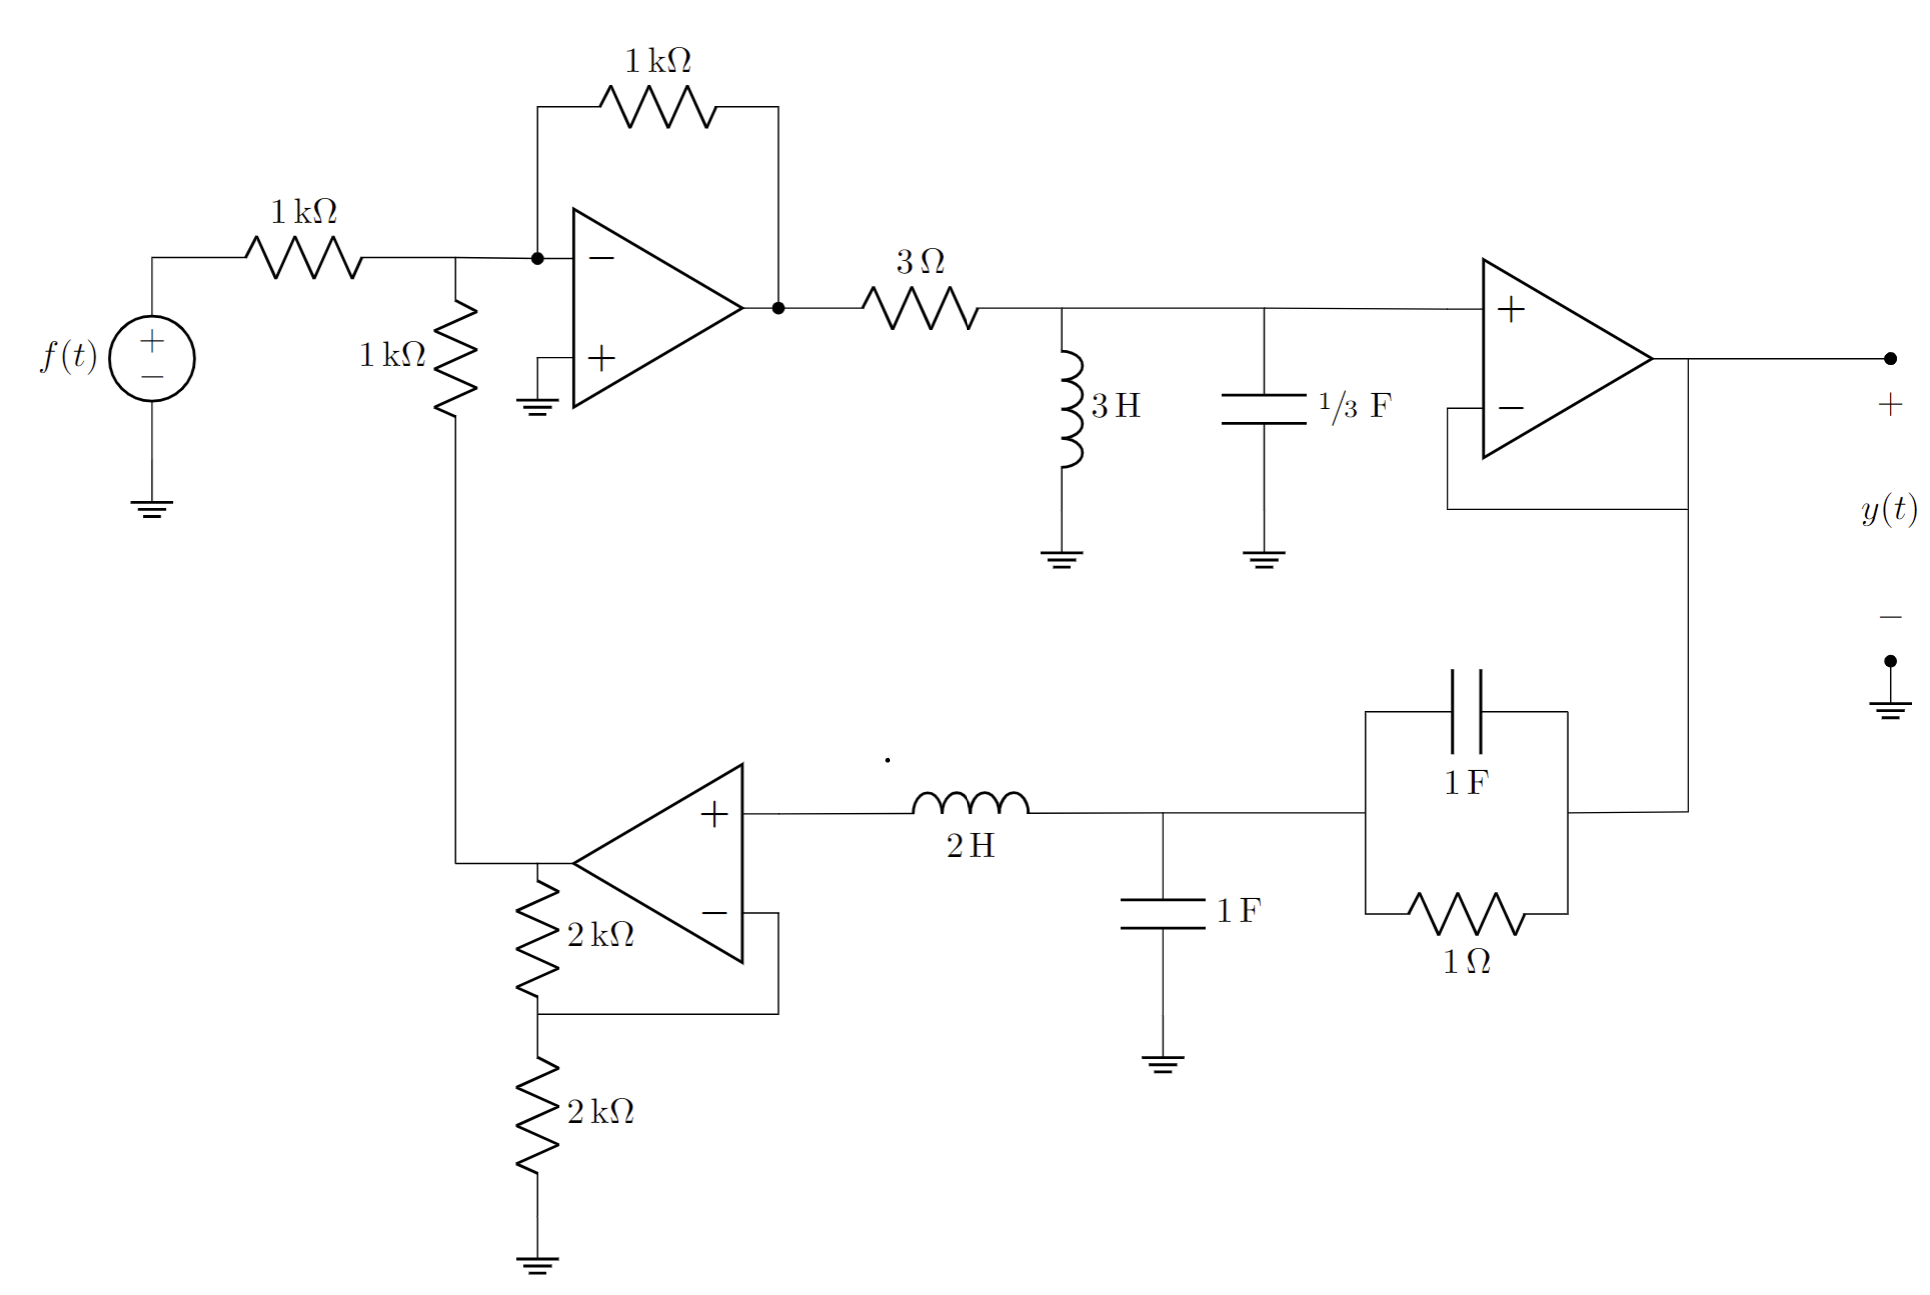
\includegraphics[width=0.75\linewidth]{figures/mega.png}
\end{figure}

\subsection{Solution}

It might not be immediately obvious looking at the circuit, but this is a 'simple' feedback system, except instead of blocks, each system is given as it's full circuit. The first step, then, is to identify each individual section in a high-level block diagram.

\begin{figure}[ht!]
\centering
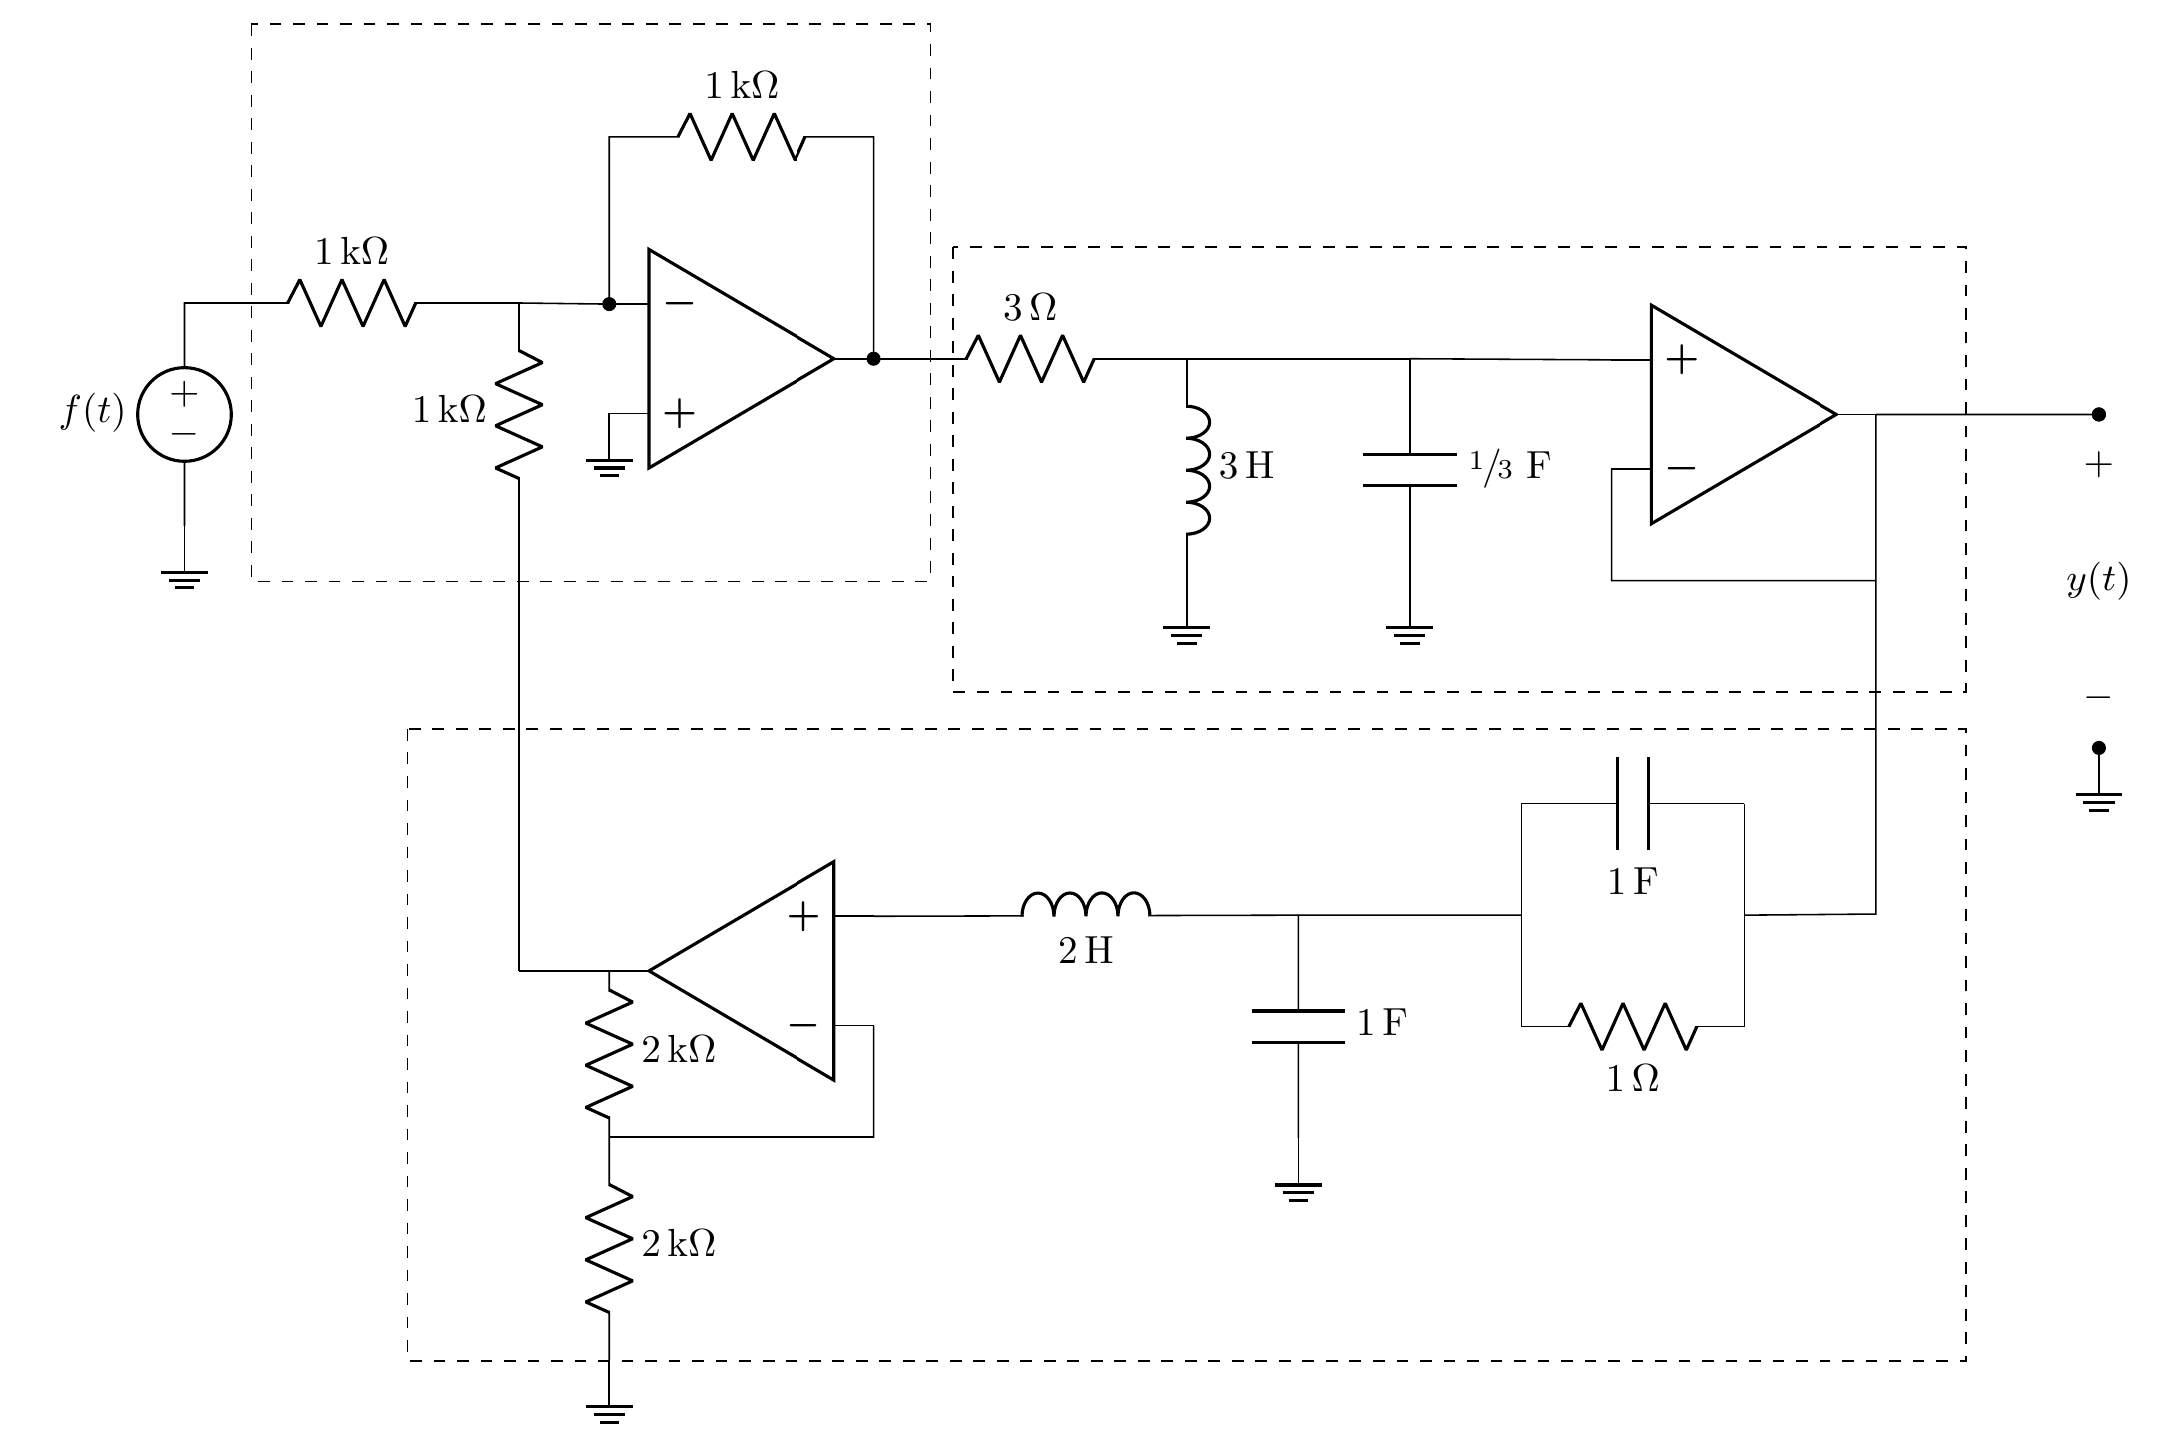
\includegraphics[width=0.75\linewidth]{figures/megabreak.png}
\end{figure}

These definitions are chosen out of convenience; other definitions are also feasible.

The top-left rectangle corresponds to an inverting adder. Consider the circuit below:


\begin{figure}[ht!]
\centering
\begin{circuitikz}[american]
	\draw  (0, 0) node[op amp] (opamp) {} 
		(opamp.-) to[short] (-2, 0.5) coordinate (feedback)
		(opamp.-) to[short,-] ++(0,1.5) coordinate (leftC) to[R=1 <\kohm>] (leftC -| opamp.out) to[short,-*] (opamp.out)
		(opamp.-) to[short] ++(-1.5,0) coordinate (minus)
		(opamp.+) to ++(0,0) node[ground]{}
		;
	\draw (minus) to[R = 1<\kohm>, -*] ++(0,-2) coordinate(i2);
	\draw (minus) to[R = 1<\kohm>, -*] ++ (-2,0) coordinate(i1);
	\node at (i1) [anchor = east] {$v_1$};
	\node at (i2) [anchor = north] {$v_2$};
	\node at (opamp.out) [anchor = west] {$v_o$};
\end{circuitikz}
\end{figure}

Since ideal op-amps have infinite input impedance, there is no current flowing into the inverting input. Now, we can set up a simple KCL equation to solve for $v_o$;

\[I_{in} = I_{out} \implies \frac{v_1 - v_-}{1000} + \frac{v_2 - v_-}{1000} = \frac{v_- - v_o}{1000}\]

Using the ideal op-amp approximation that $v_- = v_+$, and noting that the non-inverting input is grounded, we then get that $v_1 + v_2 = -v_o$. That is, the voltages present at each resistive end are summed together and inverted at the end of our op-amp. 
\vspace{5mm}

As such, we can collapse the large circuit into the following...

\begin{figure}[ht!]
\centering
\begin{circuitikz}[american]
\draw (0,0) circle (5mm);
\node at (0,0)[anchor = mid]{-$\Sigma$};
\draw (0.5,0) -- (1,0);
\draw (1,-0.5) -- (1,0.5) -- (2.5,0.5) -- (2.5,-0.5) -- (1,-0.5);
\draw (1,-1.5) rectangle (2.5,-2.5);
\draw (2.5,0) -- (3,0)[-latex] -- (3,-1);
\draw (3,-1) -- (3,-2)  -- (2.5,-2);
\draw (1,-2) -- (0,-2)[-latex] -- (0,-1); 
\draw (0,-1) -- (0,-0.5);
\node at (1.75,0) [anchor = mid]{$H_1$};
\node at (1.75,-2) [anchor = mid]{$H_2$};
\draw (3,0) to[short, *-] (3.5,0) ;
\node at (4,0) [anchor=mid]{$y(t)$};
\node at (-1.75,0) [anchor=mid] {$f(t)$};
\draw (-1.25,0) to[short] (-0.5,0);
\end{circuitikz}
\end{figure}

...where each block corresponds to a boxed section in the large circuit. Now, we need to find the transfer functions $H_1$ and $H_2$. We start with $H_1$:

\begin{figure}[ht!]
\centering
\begin{circuitikz}[american]
	\node at (0.5,0) [anchor = mid] {$v_{in}$};
	\draw (1,0) to[open] (1,0) coordinate (opamp.out);
	\draw (opamp.out) to[R=3<\ohm>] (4,0) to[L = 3<\henry>] (4,-2) node[ground]{};
	\draw (4,0) to[short] (6,0) to[C] (6,-2) node[ground]{};
	\draw (9,-0.5) node[op amp, noinv input up] (amp2) {}
		(amp2.-) to [short] ++(0,-1) coordinate (lC2) to[short] (lC2 -| amp2.out) coordinate(sys2start) to[short] (amp2.out)
	;
	\draw(6,0) to[short] (amp2.+);
	\node at (6.9,-1) [anchor=mid] {$\sfrac{1}{3}$ F};
	\draw (amp2.out) to[short] ++ (0.5,0) to[open] ++ (0.5,0) coordinate (vout);
	\node at (vout) [anchor = mid] {$v_{out}$};
\end{circuitikz}
\end{figure}

The op-amp at the end of this system is a buffer - it ensures that the transfer function of the system does not change irrespective of whatever load we place on this. Deriving this is a quick application of op-amp approximations - whatever voltage is fed into the non-inverting terminal will appear at the inverting terminal, and since this is shorted to the output, it will also appear at the output terminal of the op-amp. This is irrespective of whatever is attached at the output, so long as our inverting terminal is shorted to the output. 
\newpage

Note that in subsequent equations, $\|$ means ``in parallel.'' 

Now we just need to calculate the transfer function from the RLC network, which ends up being:

\[
\frac{\hat{V_o}}{\hat{V_i}} = \frac{3s\|\frac{3}{s}}{3 + 3s\|\frac{3}{s}} = \frac{\frac{9}{3s + 3/s}}{3 + \frac{9}{3s + 3/s}} = \frac{s}{s^2 + s + 1}
\]

We've found $H_1$ - now we need to find $H_2$. The op-amp at the end of this second system is a non-inverting amplifier with a gain of 2; op-amp approximations tell us that the voltage between the two resistors is the same as what is fed into the inverting amplifier. Thus, the voltage at the output of the op-amp is double its input, since KCL forces a match in currents across the two 2k resistors, and thus the voltage drop from $v_o$ to the intermediate node is the same as the voltage drop from that node to ground.

\begin{figure}[ht!]
\centering
\begin{circuitikz}[american]
	\draw (0,-5.5) node[op amp, xscale=-1, noinv input up] (amp3) {};
	\draw (10,-5) to[short, -] (9,-5);
	\node at (10.5,-5) [anchor = mid] {$v_{in}$};
	\draw (9,-4) to[C=1<\farad>] (7,-4) -- (7,-6) to[R, l_=1<\ohm>] (9,-6) to (9,-4);
	\draw (7,-5) -- (5,-5) to[C, l^ = 1<\farad>] (5,-7) node[ground]{};
	\draw (5,-5) to[L = 2<\henry>, mirror] (amp3.+);
	\draw (amp3.-) to[short] ++(0,-1) coordinate(rvdiv) to[short] (rvdiv -| amp3.out) coordinate (vdiv);
	\draw (amp3.out) to[R=2<\kohm>] (vdiv) to[R =2<\kohm>] ++(0,-2) node[ground]{};
	\draw (amp3.out) to[short] ++ (-0.5,0) to[open] ++ (-0.5,0) coordinate (vout);
	\node at (vout) [anchor = mid] {$v_{out}$};
\end{circuitikz}
\end{figure}

The node voltage $v_o$ is then double the voltage across the shunt capacitor. We can ignore the inductor, since it is part of a series connection into a path with infinite impedance, and $\infty + 2s$ is, well, $\infty$. Then,

\[
\frac{\hat{V_{o}}}{\hat{V_i}} = 2\frac{1\|(1/s)}{1/s + 1\|(1/s)} = 2\frac{\frac{1}{s}}{\frac{1}{s} + \frac{1}{s+1}} = \frac{2s+2}{2s+1}
\]

It might not immediately seem correct that we have a transfer function which will have greater than 1 magnitude. Now that we have $H_1$ and $H_2$, we can calculate their 'combined' transfer function.

\vspace{3mm} The input into system $H_1$ is $-(F + YH_2)$, which means its output $Y$ is given as $-H_1(F+YH_2)$;

\[
Y = -H_1F - H_1H_2Y \implies Y(1+H_1H_2) = -H_1F \implies \frac{Y}{F} = \frac{-H_1}{1+H_1H_2} = \frac{-\frac{s}{s^2+s+1}}{1 + \frac{s}{s^2+s+1}\frac{2s+2}{2s+1}}
\]

\[
= \boxed{\frac{-s(2s+1)}{(s^2+s+1)(2s+1) + s(2s+2)} \equiv \frac{-(2s^2+s)}{2s^3 + 5s^2 + 5s + 1}}
\]

\end{document}